\chapter{Echtzeitaktualisierung durch WebSockets}
Das wohl spannendste Thema und die erste große Erweiterung dieser Arbeit ist die Echtzeitaktualisierung im Hintergrund der Web-App. Mehrere Möglichkeiten sind dafür gegeben, wobei einige besser geeignet sind als andere.

\section{Einführung in WebSockets}
Mit der HTML5-Spezifikation wurden \emph{WebSockets}, ein auf TCP basierendes Netzwerkprotokoll, eingeführt, welches eine Vollduplex, bidirektionale, Single-Socket Verbindung ermöglicht \cite[S. 7]{ws}. Eine Anfrage öffnet die Verbindung zum WebSocket Server und kann beliebig lange offen gehalten werden, wobei zu jeder Zeit Daten zwischen Client und Server ausgetauscht werden. Der erste Handshake erfolgt über HTTP/1.1 und ähnelt dem zum Aufruf einer Homepage.
\\
\begin{lstlisting}[captionpos=b, caption=HTTP Request vom Client {\cite[S. 6]{rfc6455:handshake}}]
  GET / HTTP/1.1
  Host: server.example.com
  Origin: http://www.example.com
  Sec-WebSocket-Key: 7+C600xYyb0v2zmJ69RQsw==
  Sec-WebSocket-Version: 13
  Upgrade: websocket
\end{lstlisting}

Mit \emph{Upgrade: websocket} wird signalisiert, dass der Client eine WebSocket-Verbindung zum Server aufbauen möchte. Der entsprechende WebSocket Server reagiert darauf mit dem HTTP-Statuscode \emph{101 Switching Protocols}, womit er bestätigt, dass er mit dem Wechsel des Protokolls einverstanden ist.
\\
\begin{lstlisting}[captionpos=b, caption=HTTP Response vom Server {\cite[S. 8]{rfc6455:handshake}}]
  101 Switching Protocols
  Connection: Upgrade
  Sec-WebSocket-Accept: fYoqiH14DgI+5y1EMwM2sOLzOi0=
  Upgrade: WebSocket
\end{lstlisting}

Der kryptische Schlüssel \emph{Sec-WebSocket-Accept} muss vom Server berechnet und zurückgegeben werden und zeigt damit, dass er das WebSocket Protokoll versteht. Ab diesem Zeitpunkt ist der Handshake abgeschlossen und die WebSocket-Verbindung wurde aufgebaut.\par

\begin{figure}[!ht]
	\centering
	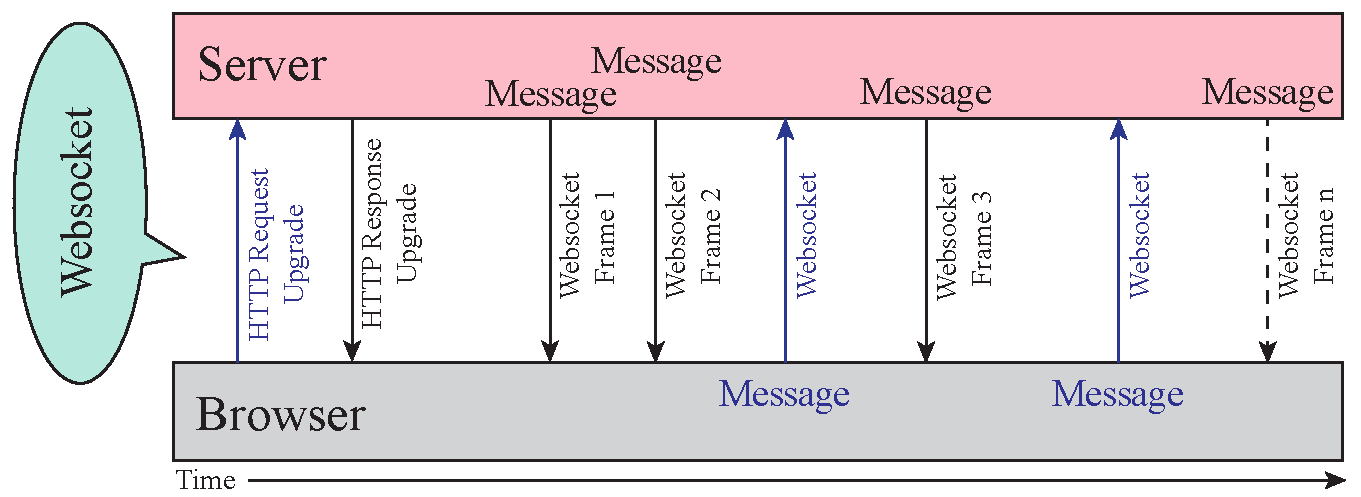
\includegraphics[width=15cm]{fig/websockets}
	\caption[Aufbau einer WebSocket Verbindung]{Aufbau einer WebSocket Verbindung. Danach können beliebig Nachrichten in beide Richtungen (gleichzeitig) übermittelt werden}
\end{figure}

Nun kommen die Vorteile von WebSockets zur Geltung: nach erstmaligem Aufbau der Verbindung bleibt diese geöffnet und zu jedem Zeitpunkt können Client und Server die Vollduplex Verbindung nutzen, um Daten miteinander auszutauschen. Das verringert Latenzzeiten (die Pakete werden direkt zugestellt, da der Server auf keinen Request vom Client warten muss), den Traffic (der Overhead ist deutlich geringer, nur ein Handshake zu Beginn erforderlich) und die CPU-Leistung der Server (der Austausch der Daten ist einfacher gestaltet als beim Polling o.Ä.).

\section{Implementierung der Echtzeitaktualisierung}
Im ersten Ansatz dieser Arbeit wurde der WebSocket-Server auf Basis von \emph{node.js} \cite{node.js}, einem serverseitigem JavaScript Framework für Server, implementiert. Das verlief aufgrund der einfachen Handhabung von WebSockets und der guten Unterstützung von HTML5 problemlos. Jedoch wurden zu diesem Zeitpunkt weder verschlüsselte Verbindungen noch Broadcasting unterstützt. Daher war dies ungeeignet, weil sensible Daten, wie die Standorte der Clients, nicht im Klartext verschickt werden sollten.\\
Außerdem ist ein Broadcast-Funktion notwendig, die den bestehenden Sockets bei Aktualisierung einer Position sofort die neuen Koordinaten übermittelt.\par

Die Implementierung beider Funktionen hätte den Rahmen dieser Arbeit überschritten, weshalb serverseitig das Open Source Modul \emph{socket.io} \cite{socket.io} für node.js verwendet wird, welches sämtliche benötigten Dienste bereitstellt und dabei noch einen Fallback zur Verfügung stellt, wodurch auch älteren Browsern ohne HTML5 Unterstützung eine websocketähnliche Verbindung ermöglicht wird.\par

Clientseitig wurde eine Routine in JavaScript entwickelt, welche im Hintergrund der Web-App ausgeführt wird. Dieses Skript verbindet sich mit dem WebSocket Server, schickt initial die aktuellen Koordinaten (unabhängig davon, welcher View gerade angezeigt wird) und wartet auf eingehende Nachrichten oder auf eine Änderung der eigenen Position. Bewegt sich der Client werden automatisch die Koordinaten GoogleMaps-kompatibel in Form von Latitude und Longitude an den WebSocket Server übermittelt.\\
Erhält der Server so eine Nachricht, aktualisiert er seine Datenbank von Standorten der Clients und schickt per Broadcast eine Nachricht an alle verbundenen Clients. So erhalten die Endgeräte in Echtzeit eine Aktualisierung aller Positionen.\par

Beendet ein Client die Verbindung oder erhält der Server keine Aktualisierungen mehr, so wird sein letzter Standort noch 15 Minuten gespeichert und dann auf allen Endgeräten gelöscht. Zu keiner Zeit werden Daten protokolliert oder länger als nötig aufbewahrt.\par

\paragraph{Entwicklung eines eigenen Protokolls zur Kommunikation über WebSockets.}
Um bestimmte Funktionen auf dem Server anzusprechen, wurde ein einfaches Protokoll entwickelt, welches angibt, um welchen Inhalt es sich bei der Nachricht handelt. So haben alle Nachrichten, die zwischen Client und Server ausgetauscht werden, ein bestimmtes Format und ein Feld \emph{type}, welches aktuell folgende Werte annehmen kann:

\begin{itemize}
	\item[] \emph{location:} enthält Latitude und Longitude des Clients
	\item[] \emph{syn:} enthält eine Signatur, die überprüft wird
	\item[] \emph{subscribe:} abonniert bestimmte Events, dazu später mehr
	\item[] \emph{publish:} signalisiert eine Änderung an der Datenbank
	\item[] \emph{message:} eine neue Chat Nachricht hat den Server erreicht und wird per Broadcast an die Clients verschickt
	\item[] \emph{history:} Anfrage eines Clients nach der aktuellen Historie des Chats
\end{itemize}

Der socket.io Server wertet diese Fälle über ein \emph{Switch-Case-Statement} aus und ruft entsprechende Methoden zur weiteren Verarbeitung auf.

\section{Authentifizierung eines Clients beim WebSocket Server}
Der Server für diese Webanwendung besteht wie beschrieben aus zwei Teilen: Apache Webserver und der socket.io WebSocket Server. Um zu beiden Servern zu verbinden sind zwei verschiedene HTTP Requests erforderlich. Bei der Webanwendung mit dem Apache kann mit einem normalen Formular der Benutzername und das Passwort eingegeben werden, allerdings hat der WS Server keinen Zugang zur Datenbank. Es muss aber eine Authentifizierung am WebSocket Server stattfinden, damit nur Benutzer aus der Webanwendung eine Verbindung erstellen können. Dafür wird das \emph{RSA Kryptosystem} verwendet.

\paragraph{Erzeugung der Schlüssel}
Bei der ersten Initialisierung der Webanwendung erstellt die App sich selbst mittels RSA Verfahren einen privaten $K^-_A$ und einen öffentlichen $K^+_A$ Schlüssel. Diese liegen beide auf dem Server wobei der öffentliche Schlüssel dem WebSocket Server bereitgestellt wird.

\paragraph{Signieren der Nachricht und anschließende Authentifizierung}
Wenn sich nun ein Client in der Webanwendung mit Benutzernamen und Passwort einloggt, nimmt die App diese Nachricht $m$ und erstellt mit dem privaten Schlüssel eine Signatur $K^-_A(m)$, welche dem Client zur Verfügung gestellt wird. Damit kann dieser nun einen syn-Request mit Benutzernamen, Passwort und Signatur an den WebSocket Server schicken. Der WS Server überprüft nun die Signatur mit dem öffentlichen Schlüssel $K^+_A(K^-_A(m))$ und wenn diese der ursprünglichen Nachricht entspricht, ist der Client authentifiziert.

\begin{figure}[!ht]
	\centering
	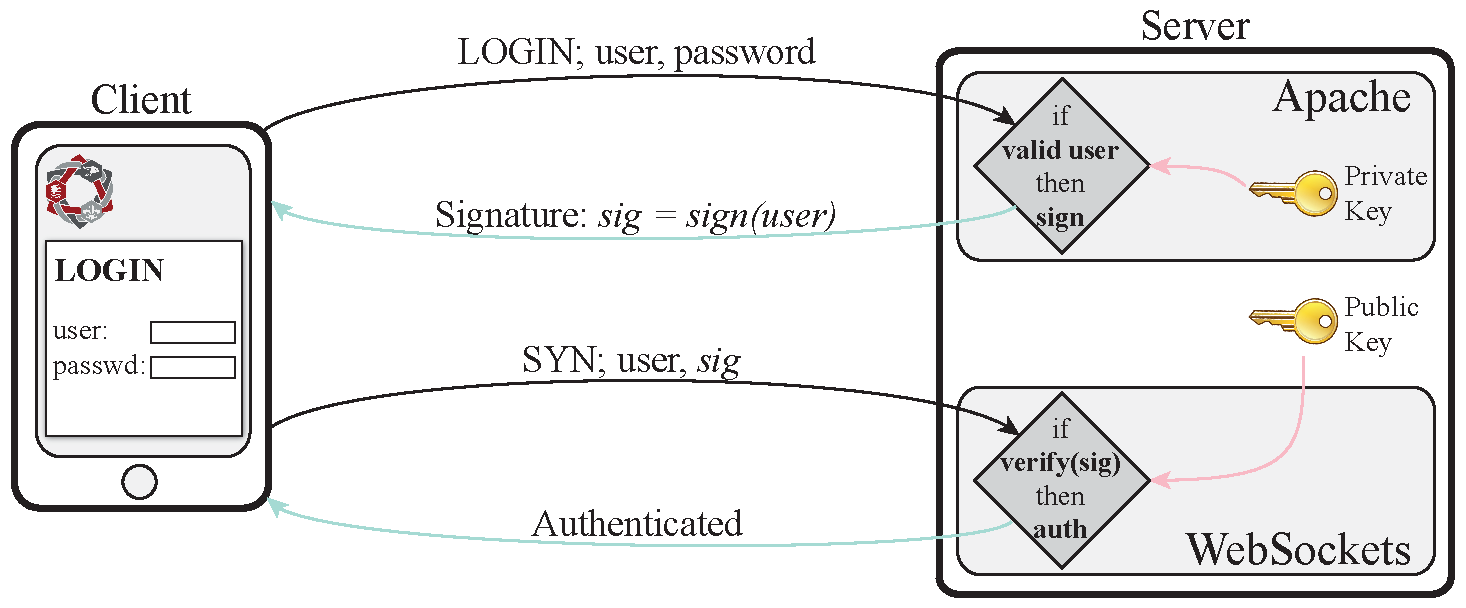
\includegraphics[width=15cm]{fig/publicprivate}
	\caption{Authentifizierung eines Clients beim Server}
\end{figure}

\paragraph{Vorteile dieser Implementierung}
Durch diese Authentifizierung kann socket.io alle eingehenden Verbindungen ablehnen, die keine korrekte Signatur erhalten haben. Ein Angreifer muss somit über den Benutzernamen und das Passwort eines Benutzers verfügen, um sowohl zu der Webanwendung als auch zum WS Server einen Zugang zu erhalten. Er kann nun aber nicht mehr ohne diese Daten eine Verbindung aufbauen und Daten abgreifen.\par

Dieser Weg der Authentifizierung wurde so gewählt, da zum Zeitpunkt des Logins der WebSocket des Endgeräts noch nicht bekannt ist. Also kann der Apache dem WS Server nicht mitteilen, welcher Benutzer zu welchem WebSocket gehört. Ein zweiter Schritt zur endgültigen Authentifizierung über eine Signatur ist also notwendig für die korrekte Zuordnung vom offenen WebSocket zum Benutzer. 

\section{Vor HTML5: Benutzung von Polling}
Für den Datenverkehr von Internetseiten wird HTTP benutzt, welches die wechselseitige Datenübermittlung \emph{Halbduplex} verwendet. So erfolgt der Datenverkehr nur in eine Richtung zur gleichen Zeit: der Client schickt eine Anfrage an den Server und dieser übermittelt danach die Antwort \cite[S. 5]{ws}. Das hat wiederum zur Folge, dass es relativ ineffizient ist, da man mit jeder Anfrage stets die Antwort des Servers abwarten muss.\par

\begin{figure}[!ht]
	\centering
	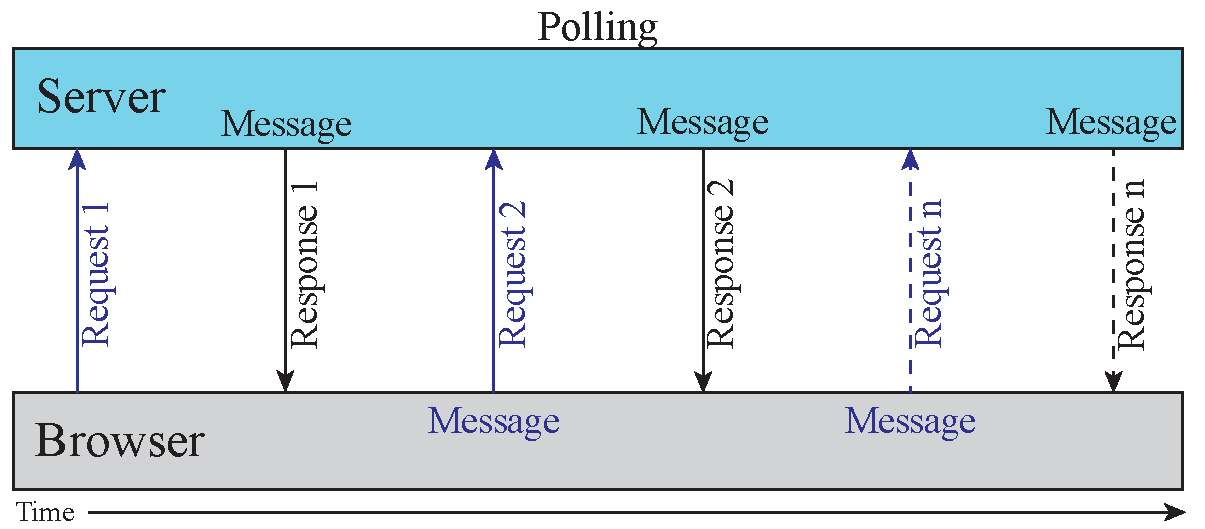
\includegraphics[width=15cm]{fig/polling}
	\caption[Datenaustausch beim Polling]{Datenaustausch mittels HTTP Request / Response beim Polling {\cite[S. 7]{ws}}}
\end{figure}

Vor diesem technischen Hintergrund wurde Polling entwickelt, bei dem in einem zeitlich bekannten Intervall eine Anfrage an den Server geschickt wird mit der Bitte um Aktualisierung. Diese Technik ist sehr attraktiv, wenn die zeitlichen Abstände der Aktualisierung der Daten bekannt ist, allerdings sind Echtzeitdaten schlecht vorhersehbar. Dadurch ist Polling nicht die richtige Wahl für dieses Projekt, weil es auf eine wirkliche Echtzeitaktualisierung ankommt.